\chapter{Resultados}

En este capitulo se presentan los distintos resultados de este trabajo de memoria.

\section{Mapeo de articulaciones}

\begin{figure}[H]
  \centering
  \begin{subfigure}[b]{0.35\textwidth}
    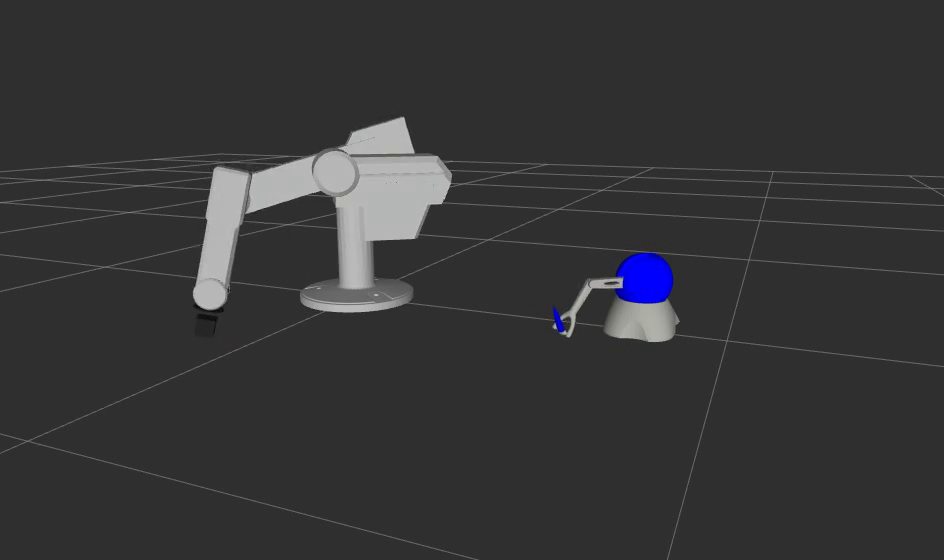
\includegraphics[width=0.9\textwidth]{img/cap5/mapping_01}
    \caption{}
  \end{subfigure}%
  \quad
  \begin{subfigure}[b]{0.35\textwidth}
    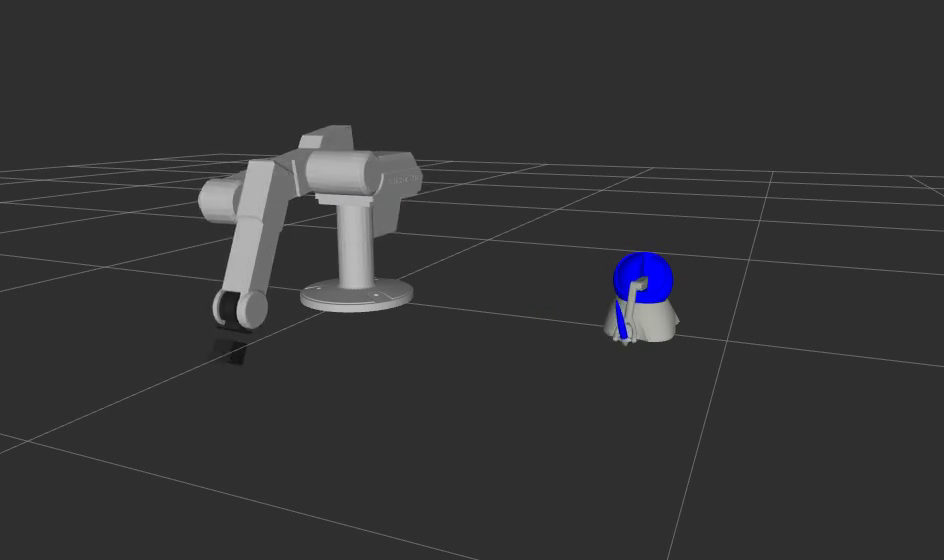
\includegraphics[width=0.9\textwidth]{img/cap5/mapping_02}
    \caption{}
  \end{subfigure}
  \vskip\baselineskip
  \begin{subfigure}[b]{0.35\textwidth}
    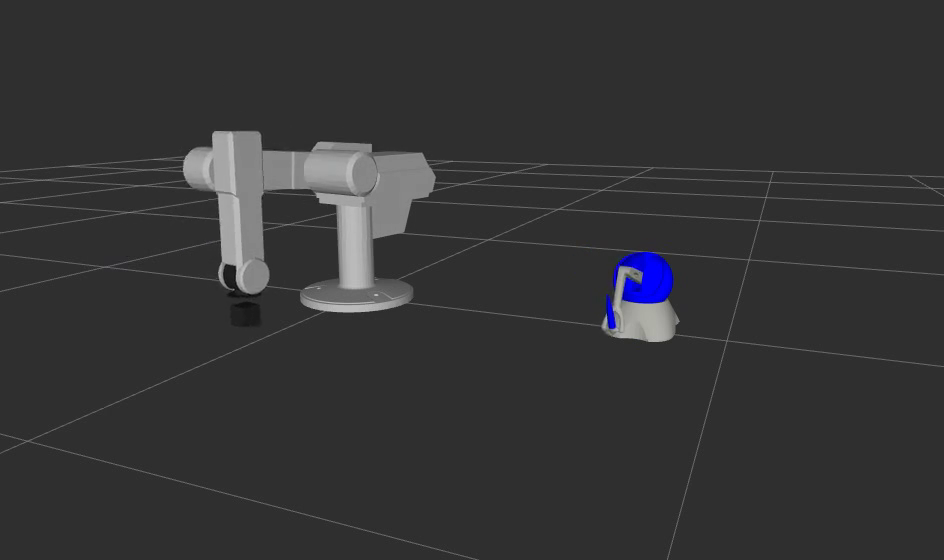
\includegraphics[width=0.9\textwidth]{img/cap5/mapping_03}
    \caption{}
  \end{subfigure}%
  \quad
  \begin{subfigure}[b]{0.35\textwidth}
    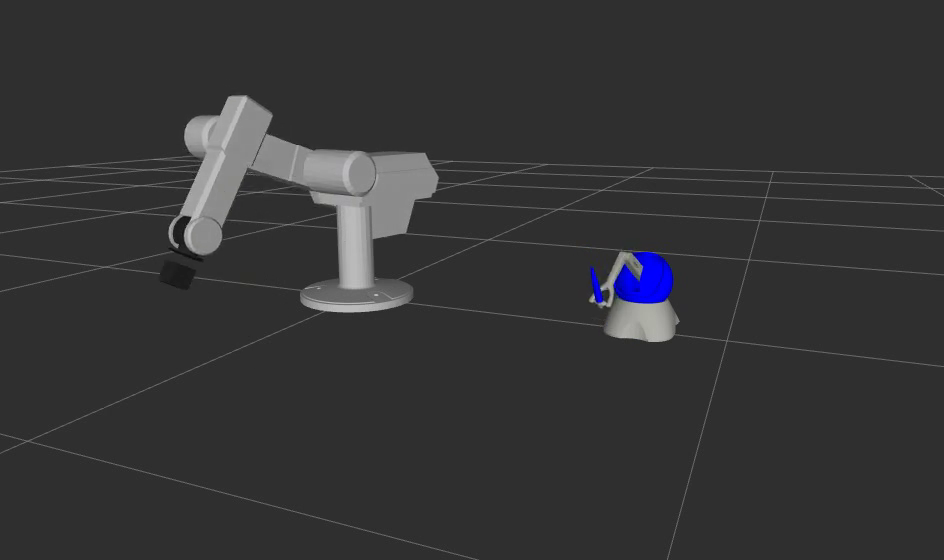
\includegraphics[width=0.9\textwidth]{img/cap5/mapping_04}
    \caption{}
  \end{subfigure}
  \caption{Mapeo de articulaciones entre el Phantom Omni y el robot Scorbot.}
  \label{cap5_joint_mapping}
\end{figure}


\begin{figure}[H]
  \centering
  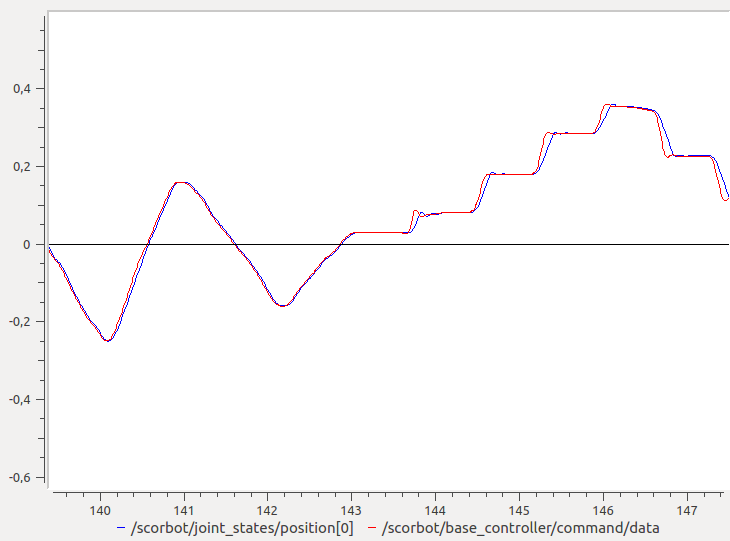
\includegraphics[width=0.5\textwidth]{img/cap5/tracking}
  \caption{Seguimiento de posición.}
  \label{cap5_pos_tracking}
\end{figure}

\begin{figure}[H]
  \centering
  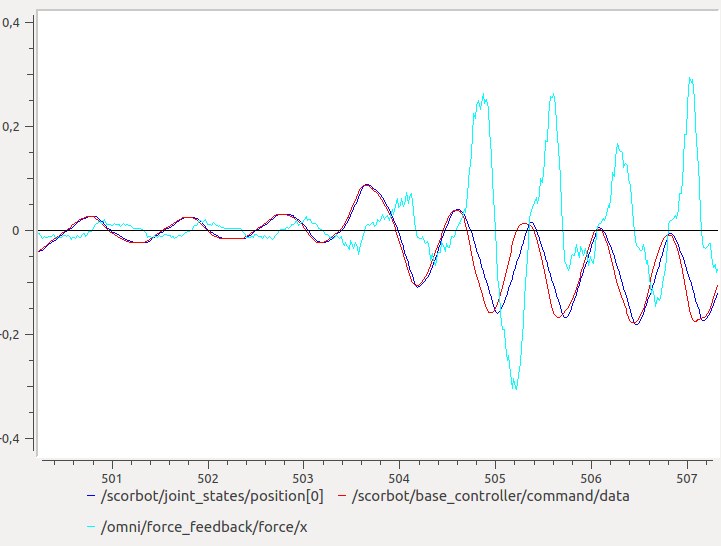
\includegraphics[width=0.5\textwidth]{img/cap5/force_feedback}
  \caption{Algoritmo de fuerza.}
  \label{cap5_force_feedback}
\end{figure}



\begin{figure}[H]
  \centering
  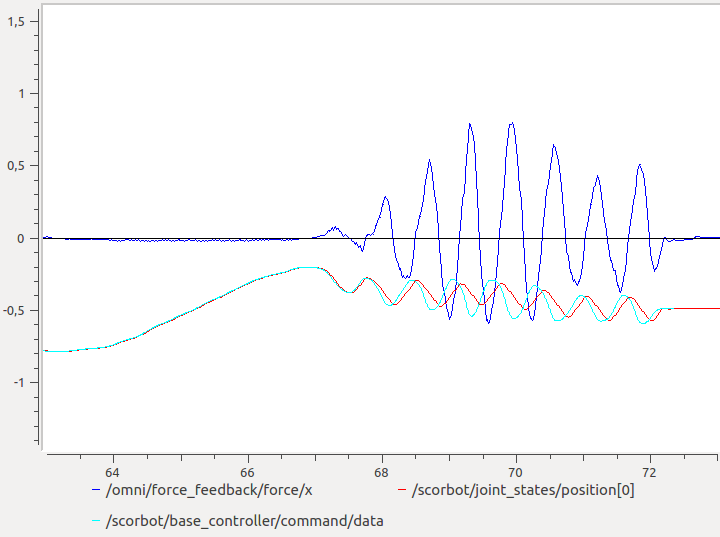
\includegraphics[width=0.5\textwidth]{img/cap5/force_tracking}
  \caption{Seguimiento de trayectoria con aplicación de fuerza.}
  \label{cap4_force_tracking}
\end{figure}


